\documentclass[11pt]{article}
\usepackage[margin=18mm,headheight=22pt]{geometry}
\usepackage{amsmath}
\usepackage{fontspec}
\usepackage{unicode-math}
\setmainfont{NewCM10}[Extension=.otf,UprightFont=*-Book,BoldFont=*-Bold,ItalicFont=*-BookItalic,BoldItalicFont=*-BoldItalic]
\setsansfont{NewCMSans10}[Extension=.otf,UprightFont=*-Book,BoldFont=*-Bold,ItalicFont=*-BookOblique,BoldItalicFont=*-BoldOblique]
\setmathfont{NewCMMath-Book.otf}
\usepackage{xcolor}
\definecolor{FAUblue}{HTML}{04316A}
\definecolor{Paperblue}{HTML}{EEF2F7}
\definecolor{EEIgold}{HTML}{CC9C42}
\usepackage{etoolbox,enumitem,booktabs,tabularx,array,needspace,microtype}
\usepackage[most]{tcolorbox}
\usepackage{titlesec,fancyhdr}
\usepackage[hidelinks]{hyperref}
\usepackage{draftwatermark}
\SetWatermarkText{Made by Thanate Amornjiraporn (Focus)}
\SetWatermarkColor{black!7}\SetWatermarkFontSize{30pt}\SetWatermarkAngle{45}
\setlength{\parindent}{0pt}
\setlength{\parskip}{5pt}
\setlist{itemsep=2pt,topsep=3pt,leftmargin=1.6em,beginpenalty=10000,endpenalty=10000}
\raggedbottom
\clubpenalty=10000 \widowpenalty=10000 \displaywidowpenalty=10000 \interlinepenalty=10000
\setcounter{secnumdepth}{0}
\setcounter{tocdepth}{1}
\pagestyle{fancy}\fancyhf{}
\fancyhead[L]{\small\sffamily\color{FAUblue} From Fundamentals to AI Apocalypse · EEI · Exercise 2}
\fancyhead[R]{\small\sffamily Exercise 2: Worked solutions}
\fancyfoot[C]{\small\thepage}
\titleformat{\section}{\Large\bfseries\sffamily\color{FAUblue}}{}{0pt}{}
\titleformat{\subsection}{\large\bfseries\sffamily\color{FAUblue}}{}{0pt}{}
\titlespacing*{\section}{0pt}{16pt}{6pt}
\preto\section{\Needspace{8\baselineskip}}
\preto\subsection{\Needspace{6\baselineskip}}
\newtcolorbox{equationcard}[1]{colback=Paperblue,colframe=Paperblue,boxrule=0pt,arc=0pt,left=10pt,right=10pt,top=6pt,bottom=6pt,title={#1},fonttitle=\small\bfseries\sffamily,coltitle=FAUblue,before skip=8pt,after skip=8pt}
\newtcolorbox{workedbox}[1]{colback=white,colframe=EEIgold,boxrule=0pt,leftrule=3pt,arc=0pt,left=10pt,top=4pt,bottom=4pt,title={#1},fonttitle=\small\bfseries\sffamily,coltitle=FAUblue,attach title to upper={\par},before skip=8pt,after skip=8pt}
\newtcolorbox{recallbox}[1]{colback=white,colframe=FAUblue,boxrule=0pt,leftrule=3pt,arc=0pt,left=10pt,top=4pt,bottom=4pt,title={#1},fonttitle=\small\bfseries\sffamily,coltitle=FAUblue,attach title to upper={\par},before skip=8pt,after skip=8pt}
\usepackage{environ}
\newsavebox\measurebox
% Typeset the section once invisibly to measure it; start a new page if it will not fit in what is left.
\makeatletter
\newif\ifkeep@measuring
\NewEnviron{keepsection}{%
  \ifkeep@measuring \BODY \else
    \edef\keep@sec{\the\value{section}}\edef\keep@sub{\the\value{subsection}}%
    \setbox\measurebox\vbox{\hsize\linewidth\keep@measuringtrue\def\Needspace##1{}\BODY}%
    \setcounter{section}{\keep@sec}\setcounter{subsection}{\keep@sub}%
    \dimen2=\ht\measurebox \advance\dimen2\dp\measurebox
    \dimen@=\textheight
    \ifdim\pagegoal<\maxdimen
      \dimen@=\pagegoal \advance\dimen@-\pagetotal
      \ifdim\dimen2>\dimen@ \clearpage \dimen@=\textheight \fi
    \fi
    % if it fits, nothing inside may force an early break
    \ifdim\dimen2>\dimen@ \BODY \else \begingroup\def\Needspace##1{}\BODY\endgroup \fi
  \fi}
\makeatother
\newtcolorbox{notebox}{colback=Paperblue,colframe=Paperblue,boxrule=0pt,arc=0pt,left=8pt,right=8pt,top=4pt,bottom=4pt,before skip=6pt,after skip=6pt}
\newtcolorbox{plainbox}{colback=white,colframe=FAUblue,boxrule=0pt,leftrule=3pt,arc=0pt,left=10pt,right=8pt,top=4pt,bottom=4pt,before skip=6pt,after skip=8pt}
\usetikzlibrary{arrows.meta}
\title{\sffamily\bfseries\color{FAUblue}Exercise 2: Worked solutions}
\author{Electrical Engineering I \ensuremath{\cdot} Module 92315 \ensuremath{\cdot} Exercise 2\\[2pt]\small From Fundamentals to AI Apocalypse · personal study guide}
\date{}
\begin{document}
\maketitle
\begingroup\footnotesize\setlength{\parskip}{0pt}\tableofcontents\endgroup
\clearpage

\Needspace{8\baselineskip}
{\large Try each part before opening the answer. The steps build fields and forces from direction and distance, then check against symmetry, units, or a limiting case.}


\begin{keepsection}
\Needspace{10\baselineskip}
\section{Task 4: Electric force compared with gravity}

\Needspace{7\baselineskip}
Protons at A carry \textit{Q}\textsubscript{A} = +1 C and electrons at B carry \textit{Q}\textsubscript{B} = \ensuremath{-}1 C; they are 1 km apart. Find |\textit{F}\textsubscript{E}|/|\textit{F}\textsubscript{G}|. Use \textit{γ} = 6.667 \ensuremath{\times} 10\textsuperscript{\ensuremath{-}11} m\textsuperscript{3} kg\textsuperscript{\ensuremath{-}1} s\textsuperscript{\ensuremath{-}2}, \textit{e} = 1.602 \ensuremath{\times} 10\textsuperscript{\ensuremath{-}19} C, \textit{m}\textsubscript{p} = 1.672 \ensuremath{\times} 10\textsuperscript{\ensuremath{-}27} kg and \textit{m}\textsubscript{e} = 9.1094 \ensuremath{\times} 10\textsuperscript{\ensuremath{-}31} kg.

\textbf{Connected topic:} Coulomb’s law (§1.2) gives the electric force; compare it with the supplied gravitational law.

\begin{keepsection}
\Needspace{7\baselineskip}
\subsection{4: Magnitude ratio}

\Needspace{4\baselineskip}
Try first: convert each 1 C charge quantity into a number of elementary charges, then form both force magnitudes before dividing.

\nopagebreak[4]{\small\itshape Answers: see “Task 4: Electric force compared with gravity” under Answers at the end.}
\end{keepsection}
\end{keepsection}

\begin{keepsection}
\Needspace{10\baselineskip}
\section{Task 5: Field from two charges on the y-axis}

\Needspace{7\baselineskip}
Place \textit{Q}\textsubscript{1} at (0, \textit{a}) and \textit{Q}\textsubscript{2} at (0, \ensuremath{-}\textit{a}). Find the field throughout the \textit{xy}-plane and simplify it on the \textit{x}-axis for the stated charge choices. With charges in coulombs and lengths in metres, field values are in N/C.

\Needspace{9\baselineskip}
\textbf{Connected topics:} Electric field strength (§1.3) defines one source field; superposition (§1.4) adds them.

\Needspace{14\baselineskip}
\begin{center}
\begin{minipage}[t]{0.950\linewidth}\centering
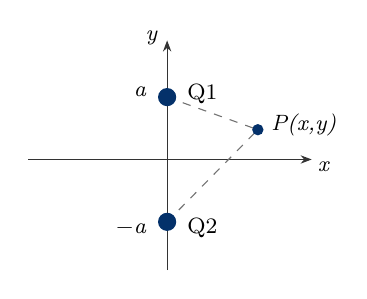
\begin{tikzpicture}
\draw[-{Stealth[length=4pt]},black!80] (0.396,-1.728) -- (3.996,-1.728);
\draw[-{Stealth[length=4pt]},black!80] (2.160,-3.132) -- (2.160,-0.216);
\draw[black!55,dashed] (2.160,-0.936) -- (3.312,-1.350);
\draw[black!55,dashed] (2.160,-2.520) -- (3.312,-1.350);
\filldraw[draw=FAUblue,fill=FAUblue] (2.160,-0.936) circle (0.108);
\filldraw[draw=FAUblue,fill=FAUblue] (2.160,-2.520) circle (0.108);
\fill[FAUblue] (3.312,-1.350) circle (0.072);
\node[anchor=west,inner sep=1pt,font=\footnotesize] at (4.032,-1.818) {\textit{x}};
\node[anchor=east,inner sep=1pt,font=\footnotesize] at (2.088,-0.180) {\textit{y}};
\node[anchor=west,inner sep=1pt,font=\footnotesize] at (2.376,-0.900) {Q1};
\node[anchor=west,inner sep=1pt,font=\footnotesize] at (2.376,-2.592) {Q2};
\node[anchor=west,inner sep=1pt,font=\footnotesize] at (3.438,-1.296) {\textit{P(x,y)}};
\node[anchor=east,inner sep=1pt,font=\footnotesize] at (1.944,-0.864) {\textit{a}};
\node[anchor=east,inner sep=1pt,font=\footnotesize] at (1.944,-2.610) {\textit{\ensuremath{-}a}};
\end{tikzpicture}\par\smallskip{\small\raggedright \textbf{Resolve each contribution from its own source.} P is arbitrary; its displacement from each charge sets direction and distance.\par}\end{minipage}
\end{center}

\begin{keepsection}
\Needspace{6\baselineskip}
\subsection{5a: Field anywhere in the plane}

\Needspace{3\baselineskip}
Try first: write the displacement from each source to P = (\textit{x}, \textit{y}), then add both vectors.

\nopagebreak[4]{\small\itshape Answers: see “Task 5: Field from two charges on the y-axis” under Answers at the end.}
\end{keepsection}

\begin{keepsection}
\Needspace{6\baselineskip}
\subsection{5b: Equal charges, Q\textsubscript{1} = Q\textsubscript{2} = Q}

\Needspace{3\baselineskip}
Try first: set \textit{y} = 0 and identify which components cancel by symmetry.

\nopagebreak[4]{\small\itshape Answers: see “Task 5: Field from two charges on the y-axis” under Answers at the end.}
\end{keepsection}

\begin{keepsection}
\Needspace{6\baselineskip}
\subsection{5c: Opposite charges, Q\textsubscript{1} = Q and Q\textsubscript{2} = \ensuremath{-}Q}

\Needspace{3\baselineskip}
Try first: again set \textit{y} = 0. Opposite signs change which components reinforce.

\nopagebreak[4]{\small\itshape Answers: see “Task 5: Field from two charges on the y-axis” under Answers at the end.}
\end{keepsection}
\end{keepsection}

\begin{keepsection}
\Needspace{10\baselineskip}
\section{Task 6: Charges at the corners of a square}

\Needspace{7\baselineskip}
Four nonzero point charges occupy corners of a square of side \textit{a}. Q is at the origin, Q\textsubscript{2} lies on the positive y-axis, and the surrounding permittivity is \textit{ε}\textsubscript{0}. With SI values, force is measured in newtons and work in joules.

\Needspace{8\baselineskip}
\textbf{Connected topics:} Coulomb’s law (§1.2) gives each force; superposition (§1.4) combines them. Work connects to electrostatic potential (§1.8).

\Needspace{14\baselineskip}
\begin{center}
\begin{minipage}[t]{0.950\linewidth}\centering
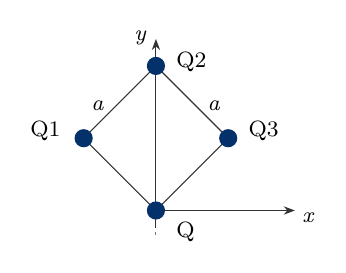
\begin{tikzpicture}
\draw[black!55,dashed] (2.160,-0.522) -- (2.160,-2.664);
\draw[black!80] (2.160,-0.522) -- (1.242,-1.440) -- (2.160,-2.358) -- (3.078,-1.440) -- cycle;
\draw[-{Stealth[length=4pt]},black!80] (2.160,-2.574) -- (2.160,-0.180);
\draw[-{Stealth[length=4pt]},black!80] (2.160,-2.358) -- (3.924,-2.358);
\filldraw[draw=FAUblue,fill=FAUblue] (2.160,-0.522) circle (0.108);
\filldraw[draw=FAUblue,fill=FAUblue] (1.242,-1.440) circle (0.108);
\filldraw[draw=FAUblue,fill=FAUblue] (3.078,-1.440) circle (0.108);
\filldraw[draw=FAUblue,fill=FAUblue] (2.160,-2.358) circle (0.108);
\node[anchor=west,inner sep=1pt,font=\footnotesize] at (2.376,-0.468) {Q2};
\node[anchor=east,inner sep=1pt,font=\footnotesize] at (0.990,-1.350) {Q1};
\node[anchor=west,inner sep=1pt,font=\footnotesize] at (3.294,-1.350) {Q3};
\node[anchor=west,inner sep=1pt,font=\footnotesize] at (2.376,-2.628) {Q};
\node[,inner sep=1pt,font=\footnotesize] at (1.422,-1.026) {\textit{a}};
\node[,inner sep=1pt,font=\footnotesize] at (2.898,-1.026) {\textit{a}};
\node[anchor=west,inner sep=1pt,font=\footnotesize] at (3.978,-2.448) {\textit{x}};
\node[anchor=east,inner sep=1pt,font=\footnotesize] at (2.088,-0.162) {\textit{y}};
\end{tikzpicture}\par\smallskip{\small\raggedright \textbf{The square is rotated in the coordinate plane.} Sloping sides are \textit{a}; the vertical diagonal Q to Q\textsubscript{2} is \ensuremath{\surd}2\textit{a}.\par}\end{minipage}
\end{center}

\begin{keepsection}
\Needspace{7\baselineskip}
\subsection{6a: Force on Q at the origin}

\Needspace{4\baselineskip}
Try first: find the source coordinates from the diagram, then resolve each force into x and y components.

\nopagebreak[4]{\small\itshape Answers: see “Task 6: Charges at the corners of a square” under Answers at the end.}
\end{keepsection}

\begin{keepsection}
\Needspace{6\baselineskip}
\subsection{6b: Condition for zero force}

\Needspace{3\baselineskip}
Try first: set both components from 6a to zero. The central charge Q is nonzero.

\nopagebreak[4]{\small\itshape Answers: see “Task 6: Charges at the corners of a square” under Answers at the end.}
\end{keepsection}

\begin{keepsection}
\Needspace{7\baselineskip}
\subsection{6c: Work to move Q\textsubscript{2} to (0, a)}

\Needspace{4\baselineskip}
Try first: with Q\textsubscript{1} = Q\textsubscript{3} = 0, compare its initial and final distance from Q. Take work as external work for a quasistatic move.

\nopagebreak[4]{\small\itshape Answers: see “Task 6: Charges at the corners of a square” under Answers at the end.}
\end{keepsection}
\end{keepsection}


\clearpage
\section{Answers}
\begin{keepsection}\subsection{Task 4: Electric force compared with gravity}

\begin{workedbox}{4 \ensuremath{\cdot} Coulomb force versus gravity}
\Needspace{13\baselineskip}
\begin{enumerate}
\item \Needspace{5\baselineskip}
Gravity needs group masses, so first convert total charge to particle count. Each particle has charge magnitude \textit{e}:

\begin{equation*}{N}\, =\, |{Q}|/{e};\, \quad \, {m}_{\mathrm{A}}\, =\, |{Q}_{\mathrm{A}}|{m}_{\mathrm{p}}/{e};\, \quad \, {m}_{\mathrm{B}}\, =\, |{Q}_{\mathrm{B}}|{m}_{\mathrm{e}}/{e}\end{equation*}
\item \Needspace{4\baselineskip}
Coulomb’s law gives electric magnitude; opposite signs make the force attractive:

\begin{equation*}|{F}_{\mathrm{E}}|\, =\, {k}|{Q}_{\mathrm{A}}{Q}_{\mathrm{B}}|/{r}_{\text{AB}}^{2},\, \quad \, {k}\, =\, 1/(4π{ε}_{0})\end{equation*}
\item \Needspace{4\baselineskip}
Insert the group masses into the given gravity relation:

\begin{equation*}|{F}_{\mathrm{G}}|\, =\, {γm}_{\mathrm{A}}{m}_{\mathrm{B}}/{r}_{\text{AB}}^{2}\, =\, {γ}|{Q}_{\mathrm{A}}{Q}_{\mathrm{B}}|{m}_{\mathrm{p}}{m}_{\mathrm{e}}/({e}^{2}{r}_{\text{AB}}^{2})\end{equation*}
\item \Needspace{4\baselineskip}
Divide the magnitudes; the charge quantities and separation cancel:

\begin{equation*}|{F}_{\mathrm{E}}|/|{F}_{\mathrm{G}}|\, =\, {k\,e}^{2}/({γm}_{\mathrm{p}}{m}_{\mathrm{e}})\end{equation*}
\item \Needspace{4\baselineskip}
Substitute \textit{k} = 8.9877 \ensuremath{\times} 10\textsuperscript{9} N m\textsuperscript{2}/C\textsuperscript{2} and the given constants:

\Needspace{4\baselineskip}
\begin{equation*}|{F}_{\mathrm{E}}|/|{F}_{\mathrm{G}}|\, \approx \, 2.27\, \times \, 10^{39}\end{equation*}

\Needspace{4\baselineskip}
\textbf{Result:} electric force is about 2.27 \ensuremath{\times} 10\textsuperscript{39} times stronger in magnitude.

\textbf{Check:} the ratio is dimensionless and independent of distance since both laws vary as 1/\textit{r}\textsuperscript{2}.
\end{enumerate}
\end{workedbox}

\end{keepsection}
\begin{keepsection}\subsection{Task 5: Field from two charges on the y-axis}

\begin{workedbox}{5a \ensuremath{\cdot} General field by superposition}
\Needspace{11\baselineskip}
\begin{enumerate}
\item \Needspace{5\baselineskip}
Point each displacement from source to P by subtracting source coordinates from point coordinates:

\begin{equation*}{r}_{1}\, =\, {x\,e}_{\mathrm{x}}\, +\, ({y}\, -\, {a}){e}_{\mathrm{y}};\, \quad \, {r}_{2}\, =\, {x\,e}_{\mathrm{x}}\, +\, ({y}\, +\, {a}){e}_{\mathrm{y}}\end{equation*}
\item \Needspace{5\baselineskip}
A point-charge vector field is \textit{kQ}\textit{r}/\textit{r}\textsuperscript{3}; signed Q handles direction. Superpose the two source fields:

\begin{equation*}{E}(\mathrm{P})\, =\, {kQ}_{1}{r}_{1}/|{r}_{1}|^{3}\, +\, {kQ}_{2}{r}_{2}/|{r}_{2}|^{3}\end{equation*}
\item \Needspace{4\baselineskip}
Take the lengths from the displacement components and substitute:

\begin{equation*}{E}({x},{y})\, =\, {kQ}_{1}[{x\,e}_{\mathrm{x}}\, +\, ({y}\, -\, {a}){e}_{\mathrm{y}}]/[{x}^{2}\, +\, ({y}\, -\, {a})^{2}]^{3/2}\, +\, {kQ}_{2}[{x\,e}_{\mathrm{x}}\, +\, ({y}\, +\, {a}){e}_{\mathrm{y}}]/[{x}^{2}\, +\, ({y}\, +\, {a})^{2}]^{3/2}\end{equation*}
\item \Needspace{5\baselineskip}
\textbf{Result:} valid except at (0, \ensuremath{\pm}\textit{a}), where an ideal point-charge field is singular.

\textbf{Check:} a positive source points along its source-to-P displacement; a negative source reverses it.
\end{enumerate}
\end{workedbox}

\end{keepsection}
\begin{keepsection}\subsection{Task 5: Field from two charges on the y-axis}

\begin{workedbox}{5b \ensuremath{\cdot} Equal charges on the x-axis}
\Needspace{8\baselineskip}
\begin{enumerate}
\item \Needspace{4\baselineskip}
At P = (\textit{x}, 0), the displacements have equal lengths and opposite vertical components:

\begin{equation*}{r}_{1}\, =\, {x\,e}_{\mathrm{x}}\, -\, {a\,e}_{\mathrm{y}};\, \quad \, {r}_{2}\, =\, {x\,e}_{\mathrm{x}}\, +\, {a\,e}_{\mathrm{y}};\, \quad \, |{r}_{1}|\, =\, |{r}_{2}|\, =\, \sqrt({x}^{2}\, +\, {a}^{2})\end{equation*}
\item \Needspace{4\baselineskip}
With equal Q, vertical components cancel and horizontal components add:

\begin{equation*}{E}({x},0)\, =\, {kQ}({r}_{1}\, +\, {r}_{2})/({x}^{2}\, +\, {a}^{2})^{3/2}\, =\, 2{kQx}{e}_{\mathrm{x}}/({x}^{2}\, +\, {a}^{2})^{3/2}\end{equation*}
\item \Needspace{5\baselineskip}
\textbf{Result:} for positive Q it points +x when x \ensuremath{>} 0 and reverses for x \ensuremath{<} 0; negative Q reverses these directions.

\textbf{Check:} at x = 0 symmetry requires zero, which the expression gives.
\end{enumerate}
\end{workedbox}

\end{keepsection}
\begin{keepsection}\subsection{Task 5: Field from two charges on the y-axis}

\begin{workedbox}{5c \ensuremath{\cdot} Opposite charges on the x-axis}
\Needspace{9\baselineskip}
\begin{enumerate}
\item \Needspace{5\baselineskip}
The distances still match, but signed contributions use the difference of the displacement vectors:

\begin{equation*}{r}_{1}\, -\, {r}_{2}\, =\, -2{a\,e}_{\mathrm{y}}\end{equation*}
\item \Needspace{4\baselineskip}
Horizontal parts cancel; vertical contributions add downward:

\begin{equation*}{E}({x},0)\, =\, {kQ}({r}_{1}\, -\, {r}_{2})/({x}^{2}\, +\, {a}^{2})^{3/2}\, =\, -2{kQa}{e}_{\mathrm{y}}/({x}^{2}\, +\, {a}^{2})^{3/2}\end{equation*}
\item \Needspace{6\baselineskip}
\textbf{Result:} for positive Q it points from upper positive to lower negative: \ensuremath{-}y. Negative Q reverses it.

\textbf{Check:} at the midpoint both fields point down. Far along the axis, magnitude falls as 1/|x|\textsuperscript{3}, as for a dipole.
\end{enumerate}
\end{workedbox}

\end{keepsection}
\begin{keepsection}\subsection{Task 6: Charges at the corners of a square}

\begin{workedbox}{6a \ensuremath{\cdot} Vector sum at the origin}
\Needspace{14\baselineskip}
\begin{enumerate}
\item \Needspace{5\baselineskip}
The square’s 45° sides project equally on both axes. The other corners and their distances from Q are:

\Needspace{4\baselineskip}
\begin{equation*}\mathrm{Q}_{1}:\, (-{a}/\sqrt2,\, {a}/\sqrt2);\, \quad \, \mathrm{Q}_{2}:\, (0,\, \sqrt2{a});\, \quad \, \mathrm{Q}_{3}:\, ({a}/\sqrt2,\, {a}/\sqrt2)\end{equation*}

Side charges are distance a; Q\textsubscript{2} is distance \ensuremath{\surd}2a.
\item \Needspace{4\baselineskip}
The top charge contributes along \ensuremath{-}y for positive QQ\textsubscript{2}; its distance is \ensuremath{\surd}2a:

\begin{equation*}{F}_{2}\, =\, -{kQQ}_{2}/(2{a}^{2}){e}_{\mathrm{y}}\end{equation*}
\item \Needspace{4\baselineskip}
The side-charge unit directions from each source toward the origin give:

\begin{equation*}{F}_{1}\, =\, {kQQ}_{1}/(\sqrt2{a}^{2})({e}_{\mathrm{x}}\, -\, {e}_{\mathrm{y}});\, \quad \, {F}_{3}\, =\, -{kQQ}_{3}/(\sqrt2{a}^{2})({e}_{\mathrm{x}}\, +\, {e}_{\mathrm{y}})\end{equation*}
\item \Needspace{4\baselineskip}
Add components and factor the scale, where \textit{k} = 1/(4π\textit{ε}\textsubscript{0}):

\begin{equation*}{F}\, =\, {kQ}/{a}^{2}\, [({Q}_{1}\, -\, {Q}_{3})/\sqrt2\, {e}_{\mathrm{x}}\, -\, (({Q}_{1}\, +\, {Q}_{3})/\sqrt2\, +\, {Q}_{2}/2){e}_{\mathrm{y}}]\end{equation*}
\item \Needspace{5\baselineskip}
\textbf{Result:} this vector is the net force on Q; charge signs select attraction or repulsion.

\textbf{Check:} each term has charge product over distance squared. If Q\textsubscript{1} = Q\textsubscript{3}, symmetry removes the x-component.
\end{enumerate}
\end{workedbox}

\end{keepsection}
\begin{keepsection}\subsection{Task 6: Charges at the corners of a square}

\begin{workedbox}{6b \ensuremath{\cdot} Cancel both components}
\Needspace{9\baselineskip}
\begin{enumerate}
\item \Needspace{4\baselineskip}
Since Q \ensuremath{\neq} 0, the shared factor kQ/a² cannot make the force zero. The x-component requires:

\begin{equation*}({Q}_{1}\, -\, {Q}_{3})/\sqrt2\, =\, 0\, \quad \, ⟹\, \quad \, {Q}_{1}\, =\, {Q}_{3}\end{equation*}
\item \Needspace{4\baselineskip}
The y-component must also vanish:

\begin{equation*}({Q}_{1}\, +\, {Q}_{3})/\sqrt2\, +\, {Q}_{2}/2\, =\, 0\end{equation*}
\item \Needspace{4\baselineskip}
Use Q\textsubscript{3} = Q\textsubscript{1} and solve:

\begin{equation*}{Q}_{2}\, =\, -\sqrt2({Q}_{1}\, +\, {Q}_{3})\, =\, -2\sqrt2{Q}_{1}\end{equation*}
\item \Needspace{5\baselineskip}
\textbf{Result:} Q\textsubscript{1} = Q\textsubscript{3} and Q\textsubscript{2} = \ensuremath{-}2\ensuremath{\surd}2Q\textsubscript{1}.

\textbf{Check:} equal side charges cancel horizontally; the top charge must have the opposite sign so its vertical force balances theirs.
\end{enumerate}
\end{workedbox}

\end{keepsection}
\begin{keepsection}\subsection{Task 6: Charges at the corners of a square}

\begin{workedbox}{6c \ensuremath{\cdot} Change in electrostatic potential energy}
\Needspace{11\baselineskip}
\begin{enumerate}
\item The diagram places Q\textsubscript{2} at (0, \ensuremath{\surd}2a); the requested endpoint is (0, a). Only the interaction with Q remains. This starting position is read from the diagram.
\item \Needspace{5\baselineskip}
For two point charges, U = kQQ\textsubscript{2}/r. Quasistatic external work equals the potential-energy change:

\begin{equation*}\mathrm{W}_{\text{ext}}\, =\, Δ\mathrm{U}\, =\, {kQQ}_{2}(1/{a}\, -\, 1/(\sqrt2{a}))\end{equation*}
\item \Needspace{4\baselineskip}
Use \textit{k} = 1/(4π\textit{ε}\textsubscript{0}):

\begin{equation*}\mathrm{W}_{\text{ext}}\, =\, {QQ}_{2}/(4π{ε}_{0}{a})(1\, -\, 1/\sqrt2)\end{equation*}
\item \Needspace{5\baselineskip}
\textbf{Result:} the signed external work is positive for QQ\textsubscript{2} \ensuremath{>} 0 and negative for QQ\textsubscript{2} \ensuremath{<} 0.

\textbf{Check:} the final separation is smaller. Like charges need positive external work to move closer; unlike charges release energy.
\end{enumerate}
\end{workedbox}

\end{keepsection}

\vfill{\small Personal worked-solution guide based on the supplied EEI Exercise 2 sheet, written in my own words; no exercise text or figures are reproduced. Not an official FAU publication; check course details against current material. Made by \textbf{Thanate Amornjiraporn (Focus)}.}

\end{document}
